\section{Latensi}
\label{sec:latensi}

Latensi adalah perhitungan dari \textit{delay} dalam sebuah sistem \parencite{goodwin2023latency}, yaitu waktu ketika pengguna melakukan sesuatu hingga aksi tersebut dapat diproses. Latensi dapat berasal dari aksi apapun. Secara fisik, latensi adalah konsekuensi dari kecepatan terbatas dari interaksi fisik apapun yang dapat merambat. Kecepatan ini akan selalu kurang dari atau sama dengan kecepatan cahaya \parencite{halliday2013fundamentals}. Dengan demikian, setiap sistem fisik dengan pemisahan apapun dalam sebab dan akibatnya akan memiliki latensi terlepas dari sifat aksi yang dilakukan. Pada cakupan suatu sistem, latensi diukur dengan waktu tempuh ketika sebuah bit data dikirimkan hingga bit data pertama diterima \parencite{johansson2000impact}.

Sistem yang merespon pada aksi pengguna dengan sangat cepat (di bawah 100 milisekon) terasa lebih cair dan natural dibandingkan yang membutuhkan lebih lama \parencite{dean2013tail}. Dalam konteks penyimpanan terdistribusi, cakupan latensi utama yang akan dibahas antara lain latensi pada perangkat memori, latensi pada disk, latensi pada jaringan, dan dipertimbangkan juga latensi dari pemrosesan algoritma serta faktor lain yang dapat memengaruhi latensi.

Latensi berbeda dengan \textit{bandwidth}, \textit{throughput}, dan \textit{response time}. \textit{Bandwidth} adalah ukuran volume data yang dapat dikirim dalam satu satuan waktu. \textit{Throughput} adalah ukuran volume data sebenarnya yang dikirim dalam satu waktu. Sementara itu, response time adalah waktu dari \textit{request} dikirim hingga \textit{response} diterima \parencite{goodwin2023latency}.

\subsection{Memori}

\subsection{Latensi Disk}
\label{sec:latensi-disk}

Latensi \textit{disk} adalah latensi yang terjadi ketika mengakses perangkat penyimpanan seperti \textit{hard disk drive} (HDD) atau \textit{solid state drive} (SSD). Sistem penyimpanan memiliki perbedaan waktu yang jauh lebih lambat dibandingkan waktu akses dari modul memori utama \parencite{ng1991improving}.

\begin{figure}[ht]
	\centering
	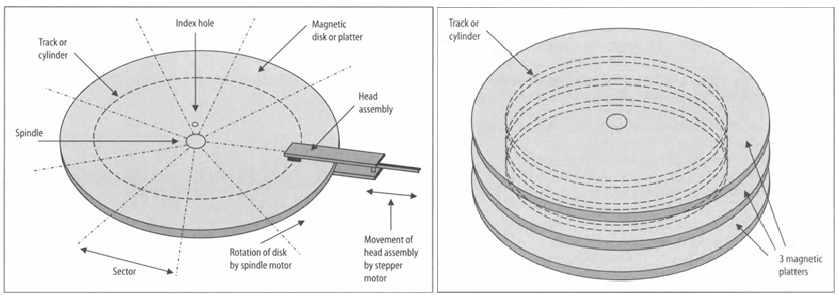
\includegraphics[width=0.95\textwidth]{resources/chapter-2/disk-structure.png}
	\caption{Struktur HDD \parencite{sammes2000disk}}
	\label{fig:hdd-structure}
\end{figure}

HDD terdiri atas susunan piringan dan penunjuk seperti yang diilustrasikan pada Gambar \ref{fig:hdd-structure}. Untuk mengakses data, pertama kali HDD harus membenarkan posisi dari kepala penunjuk sampai berada pada \textit{track} yang sesuai, waktu yang diperlukan untuk melakukan hal ini disebut dengan \textit{seek time}. Setelah kepala penunjuk sudah ada pada posisi, piringan harus berputar sampai sektor yang diperlukan berselarasan dengan kepala penunjuk tersebut, waktu ini disebut dengan \textit{rotational latency}. Karena piringan berputar terus menerus, waktu yang dibutuhkan untuk mencapai sektor yang benar bergantung pada kecepatan dari piringan tersebut. Kecepatan ini diukur menggunakan satuan \textit{rotations per minute} (RPM). Pemindahan data baru dapat dilakukan setelah kepala ada pada posisi sektor yang benar. Jika data tidak bersifat kontinu atau tersebar pada sektor yang berbeda-beda, penyesuaian kepala penunjuk dapat menyebabkan penambahan \textit{seek time} dan \textit{rotational latency} sesuai lokasi sektor tersebut. Pelaksanaan \textit{request} juga dipengaruhi oleh algoritma \textit{disk scheduling} yang digunakan \parencite{arpaci2018operating}.

Teknologi lain yang digunakan sebagai sistem penyimpanan adalah \textit{solid-state drive} (SSD). SSD tidak memiliki bagian mekanikal layaknya HDD, tetapi dibuat dari transistor seperti memori dan prosesor. Latensi dari SSD yang menggunakan teknologi \textit{flash} tidak lagi terpengaruh oleh peletakan data pada modul. Latensi berasal dari waktu yang digunakan oleh \textit{controller}. Hal yang dilakukan oleh \textit{controller} antara lain memetakan data pada blok, memanfaatkan \textit{cache} pada SSD, melakukan \textit{wear-leveling} untuk menyebar penggunaan block agar modul bertahan lebih lama, dan membersihkan dari blok yang sudah tidak terpakai. Dibandingkan dengan HDD, SSD memiliki kinerja yang jauh lebih baik dengan \textit{throughput} yang lebih tinggi dan latensi yang lebih rendah \parencite{arpaci2018operating}.

\subsection{Latensi Jaringan}

Latensi jaringan adalah waktu yang dibutuhkan untuk data menempuh jarak dari satu titik ke titik lainnya melewati jaringan. Secara teori, data dapat melintasi internet dengan kecepatan yang mendekati kecepatan cahaya. Namun, pada nyatanya, data bergerak lebih lambat sebab jarak, infrastruktur internet, ukuran paket, kemacetan jaringan, dan variabel lainnya \parencite{goodwin2023latency}. Hal ini terjadi ketika data perlu dikirim dari satu perangkat ke perangkat lainnya, misalnya pada aplikasi \textit{server} dan \textit{client}.

Pada sistem terdistribusi, latensi jaringa berperan besar terhadap \textit{response time} karena sistem terpisah dari lokasi fisik yang jauh. Hal ini disebabkan mendistribusikan data pada jaringan lokal tidak memiliki banyak guna \parencite{johansson2000impact}. Sekalipun berjarak dekat, pengiriman data antar perangkat membutuhkan waktu untuk mengirimkan data atau \textit{transmit time} dan penerimaan dari data tersebut di sisi penerima.

% \input{chapters/chapter-2/02-04-latensi-faktor-lain.tex}
